\documentclass[11pt]{article}
%\usepackage[utf8]{inputenc}
\usepackage{deauthor,times,graphicx}
\usepackage{hyperref}
\usepackage{xspace}
\usepackage{xcolor}

\newcommand{\etal}{\textit{et~al.}\xspace}
\newcommand{\eg}{\textit{e.g.}\xspace}
\newcommand{\ie}{\textit{i.e.}\xspace}
\newcommand{\aka}{\textit{a.k.a.}\xspace}
\newcommand{\etc}{etc.\xspace}
\newcommand{\cf}{cf.\/~}
\newcommand\figref[1]{Figure~\ref{#1}}
\newcommand\algref[1]{Algorithm~\ref{#1}}
\newcommand\tabref[1]{Table~\ref{#1}}
\newcommand\secref[1]{Section~\ref{#1}}
\newcommand\equref[1]{Equation~(\ref{#1})}
\newcommand{\fakeparagraph}[1]{\vspace{1mm}\noindent\textbf{#1.}}

\graphicspath{{authorname/}}

\ifodd 1
\newcommand{\rev}[1]{{\color{blue}#1}} %revise of the text
\newcommand{\TODO}[1]{{\textbf{TODO}:{ #1} }}
\newcommand{\zeng}[1]{{\color{brown}#1}} %revise of the text
\else
\newcommand{\rev}[1]{#1}
\newcommand{\TODO}[1]{}
\newcommand{\zeng}[1]{#1}
\fi

\begin{document}

\title{Federated Learning in the Lens of Crowdsourcing}
\author{
        Yongxin Tong,
        Yansheng Wang,
	    Dingyuan Shi \\
	    SKLSDE Lab, BDBC and IRI, Beihang University, China\\
		\{yxtong, arthur\_wang, chnsdy\}@buaa.edu.cn
}

\maketitle

\begin{abstract}
The success of artificial intelligence (AI) is inseparable from large-scale and high-quality data, which is not always available.
Involving human forces like crowdsourcing can help provide more training data and improve data quality for AI tasks.
But with more privacy concerns and stricter laws, the data isolation problem is becoming worse, just when federated learning (FL) has emerged as a promising solution. 
In this article, we highlight the core issues in federated learning in the lens of crowdsourcing, including privacy and security, incentive mechanism, communication optimization and quality control.
We expect to inspire the design of federated learning systems with existing crowdsourcing techniques.
We also discuss emerging future challenges to implement a fully fledged federated learning platform.
\end{abstract}

\section{Introduction}
Artificial intelligence (AI) has come to a golden age. With the help of big data, new learning algorithms and powerful computing hardware, AI has shown huge potential in many real-life applications, such as image recognition and text processing. 
However, its success highly relies on large-scale and high-quality training data, which is not always available. 

Involving human forces proves effective in either providing more training data or improving the data quality for AI tasks.
In particular, crowdsourcing \cite{DBLP:journals/tkde/ChittilappillyC16, DBLP:journals/vldb/TongZZCS20}, is one of the most practical solutions to data problems in AI. 
It is a computation paradigm where humans are gathered to collaboratively accomplish easy tasks. 
%Many sub-tasks of data processing in AI, such as labeling MRI images of brain cancers for image classification, or voting for whether Michael Jackson is a musician in a knowledge base, are intrinsically easier for humans than for computers. Therefore, crowdsourcing techniques with human participation often help deal with the data problems in AI. 
A representative example of crowdsourcing empowered AI is the famous ImageNet project \cite{DBLP:conf/cvpr/DengDSLL009}, where most pictures are labeled by crowdsourced workers. 
The Amazon Mechanical Turk (AMT) is one of the most successful commercial crowdsourcing platforms, where a large number of data labeling tasks with monetary rewards are provided by AI practitioners for freelancers. 
%Human intelligence has shown great advantages in these tasks, and brought the bonus of AI to more industrial applications.

The lack of large-scale training data is becoming more severe in recent years. 
%These challenges mainly come from the data isolation problem. 
In many industries, data are often isolated by different companies or organizations. 
Because of commercial competition and administrative issues, they would not like to share their data. 
They have to train models separately with their own data but the performance is often unsatisfactory due to the lack of data. 
Meanwhile, with people's increasing awareness on data security and individual privacy, data privacy in AI is becoming increasingly important. 
Many countries are enacting strict laws to protect the data privacy of their citizens. 
For example, EU's General Data Protection Regulation (GDPR) which was enforced on May 25, 2018, has stipulated that any use of personal data in a company must be authorized by the data owners. 
Therefore, privacy issues exacerbate the data isolation problem.

Federated learning (FL) \cite{DBLP:journals/corr/KonecnyMYRSB16, DBLP:conf/aistats/McMahanMRHA17, DBLP:journals/tist/YangLCT19} has emerged as a promising solution to the data isolation problem in AI.
First proposed by Google, FL aims to collaboratively build machine learning models with data from massive mobile devices without violating data privacy. 
As with crowdsourcing, FL also organizes humans, their devices and data, to collaborate on specific tasks. Therefore, FL can be considered as a special form of crowdsourcing. 
In this paper, we propose to understand federated learning from the lens of crowdsourcing.
The characteristics of FL in the core issues of generic crowdsourcing and the unique issues of FL are summarized as below.

\begin{figure}
\centering
\includegraphics[scale=0.5]{submissions/yongxin/figs/fig1.pdf}
%\includegraphics[scale=0.5]{figs/fig1.pdf}
\caption{Comparison between crowdsourcing and federated learning.}
\label{fig:comparison}
\end{figure}

%They have many characteristics in common while big differences also exist, which makes FL much more challenging than crowdsourcing. A brief comparison is made as below.
\begin{itemize}
	\item \textbf{Privacy and security.} 
	The most important issue in FL is privacy protection, whereas privacy is of less concerns in general crowdsourcing. 
	Secure machine learning algorithms often play a central role in FL. 
	%but is also crucial in certain scenarios like spatial crowdsourcing where the sensitive location information should not be leaked.  
	\item \textbf{Incentive mechanism.} 
	Both FL and general crowdsourcing need to motivate participants. 
	However, there are two differences. 
	The incentive mechanism in many crowdsourcing applications is based on the Business-to-customer (B2C) mode while in FL it can also be the Business-to-business (B2B) mode, as the participators in FL can be different companies. 
	The incentive procedure in crowdsourcing is often a single round, while in FL it takes multiple rounds following the training steps in machine learning, which makes the design of incentive mechanisms more difficult.
	\item \textbf{Communication optimization.} 
	In crowdsourcing the communication overhead is usually not a problem as each participant only has to submit small data (like the label of a picture) for a single round. 
	However, in FL it can be a core issue because the training process often involves frequent communication of high dimensional gradients. 
	%Many existing works on FL concentrate on reducing the communication cost, which makes it a unique challenge.
	\item \textbf{Quality control.} 
	Optimizing the collaboration results is crucial both in crowdsourcing and FL. 
	The difference is that in crowdsourcing the task is simple and the focus is to improve the accuracy of integrated results with a constrained budget. 
	The task in FL is more complicated, and the focus lies in how to deal with the heterogeneity of different parties such as non independently and identically distributed data and imbalanced computation resources.
	\item \textbf{Task assignment.} 
	Task assignment is a core component in a crowdsourcing platform \cite{DBLP:conf/icde/TongSDWC16, 8897719}, which needs to manage massive tasks and workers and to effectively allocate the resources. 
	The assignment results can decide the practical performance of the platform. 
	In FL, task assignment may not be an issue, as there is only one learning task in most cases. 
	%But a conceptional federated learning platform may also have multiple task requesters which can make task assignment meaningful. 
\end{itemize}

This paper discusses the above core issues in federated learning from the perspective of crowdsourcing.
The aim is to inspire the design of federated learning systems with existing techniques in crowdsourcing platforms. 
We also pinpoint future challenges to implement a fully fledged federated learning platform following the principles of crowdsourcing.

%An FL platform with more complete functionality can be designed following the core components in crowdsourcing. 
%We will make a vision on such a platform and conceive some future challenges.

\section{Privacy and Security}
%Although crowdsourcing also considers the privacy and security issues, their positions have been improved as never before in federated learning. 
In general crowdsourcing, workers and users only provide some necessary information such as worker skills or positions which only leaks little privacy.
Existing privacy protection techniques like anonymization and encryption are sufficient to protect such information.
However, in federated learning, the protection object becomes massive user data which is more sensitive and easier to leak privacy when external knowledge is used.
Furthermore, compared with crowdsourcing, federated learning makes it harder to judge the benignity of user uploads.
This is because machine learning models are black boxes and it is non-trivial to explain the contribution of user uploads.
Accordingly, it is possible for malicious users to upload information and thwart model training.

%also brings about new challenges in mechanism design and quality control which will be discussed in detail in \secref{sec:IncentiveMechanismDesign} and \secref{sec:QualityControl}, respectively.

A federated learning system is expected to offer periodic protection on both user data privacy and model security, as shown in \figref{fig:protection}.
Specifically, a safe-to-use federated learning framework should 
\textit{(i)} collect and use user data privately and 
\textit{(ii)} ensure that the model converges without poisoning and will not be stolen.

\begin{figure}
\centering
\includegraphics[scale=0.4]{submissions/yongxin/figs/protection.pdf}
%\includegraphics[scale=0.4]{figs/protection.pdf}
\caption{Completely periodic protection in federated learning.}
\label{fig:protection}
\end{figure}

\subsection{Data Privacy Protection}
In federated learning, for each participator, the server and other participators cannot be easily trusted. Direct uploading of raw data can lead to privacy leaks.
Uploading model parameters instead of raw data seems safer, which is also allowed in the most recognized algorithm FedAvg \cite{DBLP:conf/aistats/McMahanMRHA17}.
Some recent findings, however, show that only with model parameters, a malicious attacker can still deploy inference attack to judge membership or even reconstruct the raw data~\cite{DBLP:journals/tifs/PhongAHWM18}.
Therefore, we need to design privacy protection protocols for federated learning, which mainly include two techniques: perturbation and encryption.

\fakeparagraph{Perturbation}
Perturbation techniques require participators to inject noise to their raw data or intermediate results, making others hard to infer what they have uploaded.
To quantitatively analyze the degree of noise injection, a widely accepted measure is differential privacy (DP), proposed by Dwork~\cite{DBLP:conf/icalp/Dwork06}.
Its idea is to quantify the degree of indistinguishability by probability distributions.
The DP measurement is firstly brought up and applied in database. In the field of federated learning, however, a big challenge derives from the long iterative process and from massively distributed data. 
For each participator and in each iteration, DP should always be satisfied.
Ensuring such strict privacy protection requires strong noise to be injected, which severely deteriorates data accuracy.
To prevent privacy cost from boosting wildly with iteration rounds, moments accountant~\cite{DBLP:conf/ccs/AbadiCGMMT016} has been proposed. 
It can make the privacy budget increase sub-linearly (square root) to iteration rounds. 
As for large node numbers, shuffle model~\cite{DBLP:conf/soda/ErlingssonFMRTT19} techniques effectively cut down privacy budgets by ensuring anonymity.
Besides supervised learning, DP has also been applied to unsupervised algorithms like topic modeling \cite{DBLP:conf/cikm/JiangSTWZXY19, DBLP:conf/aaai/WangTS20}.
%Apart from the above theoretical works to ensure the data availability, we also need more practical approaches. A combination of differential privacy and ADMM, a large-scale distributed machine learning algorithm, is then proposed in \cite{DBLP:journals/tifs/HuangHGCG20}.

\fakeparagraph{Encryption}
Perturbation technique can be considered as a balance between privacy levels and data accuracy. Nevertheless, perfect secrecy cannot be achieved as exposure of little private information always exists. 
Encryption techniques, on the other hand, aim to directly circumvent such exposure, \ie, to calculate via ciphertexts. Several existing encryption techniques can be applied to federated learning, such as secure multiparty computation (SMC), homomorphic encryption (HE) and garbled circuits (GC).
Bonawitz et al use pseudo random vectors as a mask to cover the raw updates and those random vectors can neutralize each other after aggregation~\cite{DBLP:conf/ccs/BonawitzIKMMPRS17}.
Using HE to protect user privacy demands a protocol via which the server can aggregate the ciphertexts from each device and finally decipher the result~\cite{DBLP:journals/tifs/ErkinVTL12}.
%Embedding GC technique into HE protocol is devised to speed up the encryption process\cite{DBLP:conf/sp/NikolaenkoWIJBT13}.
Besides software level solutions, hardware solutions are also worth considering such as the trusted execution environment (TEE).

\subsection{Model Security Protection}
Model security refers to that the model converges to a global optimum and the results can be used safely.
Model security can be violated by multiple types of attacks.

\fakeparagraph{Byzantine Attack} 
Byzantine attack is a classical attack in distributed networks. Attackers aim to disturb the model training process and make the model unable to converge.
In FL, the malicious nodes (Byzantine nodes) will upload random vectors to mislead the aggregated gradient descent direction and thus obstruct the model convergence. 
The core idea to detect Byzantine attack is to evaluate and to spot the outliers among user uploads. 
Intuitively, examining the angle between different vectors' directions may be a solution ~\cite{DBLP:conf/nips/BlanchardMGS17}.
Another intuitive way is to use the distance to median values as an outlier judgement and its effectiveness is also verified in ~\cite{DBLP:conf/nips/AlistarhA018}. 
By maintaining a non-Byzantine node set while training, the later solution reaches lower time complexity. 

\fakeparagraph{Backdoor Attack} 
By deploying Byzantine attack detection techniques, we can ensure the convergence of model training. 
However, some higher-level attackers (nodes) can cheat the Byzantine detector by uploading plausible updates and force the model to converge to a point where some subtasks or intentionally designed misclassification are achieved. 
For example, the attacker may hope to make a spelling prompt model always provide some specific words (A restaurant owner hopes her restaurant name be prompted after a user types ``My favorite restaurant is...''). 
To realize this, unlike Byzantine attackers who simply upload random vectors, they will use data poisoning or model poisoning techniques. 
The purpose of data poisoning is to train models with intentionally mislabeled or polluted data while
%Biggio et al propose to generate data by gradient ascent to realize data poisoning~\cite{DBLP:conf/icml/BiggioNL12}. 
%Xie et al find that distributing contaminated data samples into several nodes instead of a single one will work better~\cite{DBLP:conf/iclr/XieHCL20}. 
model poisoning refers to that malicious nodes train and upload local models with training goals different from the global model.
%The main idea is to modify the local loss function to get an anomalous local model. 
%By setting the loss function as an average of normal training goal and anomalous training goal, model poisoning can be implemented ~\cite{DBLP:conf/aistats/BagdasaryanVHES20}.
%In order to cheat Byzantine detection, Bhagoji et al consider adding punishment terms into loss function to make the update not too far from historical updates~\cite{DBLP:conf/icml/BhagojiCMC19}. 
To tackle data or model poisoning, we can evaluate the approximated loss upper bound and remove outliers before local model aggregation~\cite{DBLP:conf/nips/SteinhardtKL17}. 
%For neural networks, we can prune those neurons which are dormant on normal inputs and then apply fine-tuning to readjust the neural network~\cite{DBLP:conf/raid/0017DG18}.
%Tran et al find that backdoor attack tends to leave behind a ``spectral signature'' on its feature covariance spectrum, then detecting the signature will help to remove the anomalous local uploads \cite{DBLP:conf/nips/Tran0M18}. 

\fakeparagraph{Model Stealing} 
Equipped with Byzantine and backdoor attack detectors, a federated learning system is able to safely train a model. However, we also need to provide protection for model use. 
Model stealing happens when the model is confidential and can only be used via APIs (\ie, Machine-Learning-as-a-Service, MLaaS). 
In that case, attackers may use the APIs to infer the model structure and parameters, and the confidential information of the model is exposed.
In federated learning, this may happen when one of the participators wants to forcibly occupy all the outcomes. To prevent this, we can deploy a detector to examine the frequency of API queries and judge whether the query sequence is benign~\cite{DBLP:conf/eurosp/JuutiSMA19}.

\section{Incentive Mechanism}
\label{sec:IncentiveMechanismDesign}
Both general crowdsourcing and FL involve multiple human participators. 
Thus suitable incentive mechanisms are necessary to attract people to actively contribute to the tasks.
%Incentive mechanism design of crowdsourcing has become increasingly mature in the past decades.
In traditional crowdsourcing, some tasks may be less attractive to workers due to distance, difficulty or other reasons.
Therefore, the platform needs to motivate the workers with additional rewards \cite{DBLP:conf/sigmod/TongWZCDY18}. 
%By designing flexible pricing mechanisms, those tasks can be finished timely\cite{DBLP:conf/sigmod/ParkW14, DBLP:journals/pvldb/GaoP14}.
%In spatial temporal crowdsourcing, new challenges arise, since pricing mechanism is designed not only to attract workers but also to incite workers to move physically as well\cite{DBLP:journals/vldb/TongZZCS20}.
%This new property adds difficulty of mechanism design.
For FL, incentive mechanism design is more difficult. 
This is because the black-box nature of many machine learning models makes it tricky to evaluate each participator's contribution. 
Furthermore, the number of participators in FL, especially in cross-device settings, can be much larger than in traditional crowdsourcing.
%Thus, to design a reasonable, effective and efficient incentive mechanism in federated learning is much more challenging. 

\begin{figure}
\centering
\includegraphics[scale=0.4]{submissions/yongxin/figs/mechanism.pdf}
%\includegraphics[scale=0.4]{figs/mechanism.pdf}
\caption{Mechanism design over all periods.}
\label{fig:mechanism}
\end{figure}

The mechanisms for FL should be incentive-compatible and fairness-aware.
They can be accomplished before, during and after training process, as shown in \figref{fig:mechanism}.

\fakeparagraph{Mechanisms before Training}
Designing mechanisms to incite participators before training means to establish suitable rules for data trading.
In the past decade several data markets and data sharing platforms such as Dawex\footnote{https://www.dawex.com}, Xignite\footnote{https://www.xignite.com} and WorldQuant\footnote{https://www.worldquant.com} have been developed.
They all hope to build a data trading platform where companies and users can buy, sell and exchange data with satisfactory prices to all parties.
However, this goal is hard to reach. As Fernandez et al point out, different combinations of data may produce different levels of values\cite{DBLP:journals/pvldb/FernandezSF20}, 
so instead of setting static price for data, people seek to find dynamic evaluation methods.

\fakeparagraph{Mechanisms during Training}
The goal of designing mechanisms during training is to incite the participators to use their best data for training. 
To achieve the goal, participators who contribute the most deserve the highest reward. Many researchers model the training process as a Stackelberg game\cite{DBLP:journals/twc/PandeyTBTMH20}.
There are two stages in this setting. In the first stage, the server receives updates from each user and distributes rewards base on their contributions to the model. In the second stage, users change their update strategies based on the rewards they receive.
Then the cycle repeats until all the server and users converge to equilibrium. 
Chen et al study mechanism design of federated learning from a game theoretical and optimization perspective.
Recent years blockchain emerges as a novel technique and raises wide-spread research enthusiasm. It is also an alternative technique to design incentive mechanisms.
One way to combine blockchain with mechanism design is to build a reputation record by the blockchain\cite{DBLP:journals/iotj/KangXNXZ19}. 
Owing to the immutability and consensus of blockchain, users' reputation would be hard to recover once it gets damaged and thus the participators will behave honestly to maintain their reputations.
%Another way is to trade data via blockchain directly\cite{DBLP:journals/iacr/WengWLZL18}. Users can upload their data and get tokens(coins) as rewards.

\fakeparagraph{Mechanisms after Training}
In cross-silo federated learning settings the companies cooperate with each other to train a global model and the rewards (profits) mainly come from the model use.
Distributing the profits fairly requires designing mechanisms that can evaluate each entity's contribution to the final model. 
Shapley value is a classical concept in game theory to evaluate contributions and can also be applied in profit sharing in federated learning.
The drawback is that the calculation of Shapley values is time-consuming. As a result, Song et al propose a novel accleration technique to make it practical\cite{DBLP:conf/bigdataconf/SongTW19}.


\section{Communication Optimization}

Crowdsourcing platforms usually do not care the communication overhead. 
Tasks like labeling the images require the workers to upload very few data for a single round. 
The workers can submit their results separately and occasionally.
Hence there is not much pressure on the server's communication bandwidth. 
However, the communication cost becomes a primary bottleneck for FL.
Model training algorithms like the stochastic gradient descent (SGD) take a large number of rounds to converge.
%In a centralized distributed learning setting, each party (or node) has to communicate with the server for each iteration during the convergence.
%The data they communicate with each other is the updating of gradients, which takes as much space as the model.
%Besides, the parties have to submit the data simultaneously to guarantee the correctness of the convergence.
%Even with an asynchronous algorithm, they cannot upload the gradients whenever they like as in crowdsourcing.
Besides, unlike the powerful servers in distributed learning, the nodes in FL are massively distributed mobile devices with limited communication bandwidth and active time, which makes the problem even more challenging.   

Many methods have been proposed to improve the communication efficiency of FL. 
Two basic ideas are to either reduce the number of interactions between parties and the server or to compress the data in transmission. 
These two ideas can also be combined.
Some representative techniques are explained as below.

\begin{figure}
\centering
\includegraphics[scale=0.4]{submissions/yongxin/figs/communication.pdf}
%\includegraphics[scale=0.4]{figs/communication.pdf}
\caption{Communication optimization techniques in federated learning.}
\label{fig:communication}
\end{figure}

\subsection{Interactive Number Reduction}

There are three different ways to reduce the number of interactions during the federated learning process: client sampling, 
%which reduces the number of participating parties in each round;
local updating, 
%which reduces the number of iterations to converge by keeping some computation locally; (iii) and 
and decentralized training.
%which applies decentralized optimizing algorithms to reduce interaction numbers. 
%We will discuss about them respectively.

\fakeparagraph{Client Sampling}
In a cross-device federated learning scenario, there are usually millions of devices in participation, which makes round-robin strategies impossible to work. 
The server has to sample some parties in each round for faster convergence and the accuracy should be compromised.
The client sampling trick usually does not work alone.
In some earliest works of FL such as Federated Optimization \cite{DBLP:journals/corr/KonecnyMR15} and FedAvg \cite{DBLP:conf/aistats/McMahanMRHA17}, random sampling over multiple parties is used during the training process. 
Afterwards, it is applied by other works on cross-device FL by default.
Most of them still use the simplest uniformly random sampling method.
Some consider choosing the clients conditionally.
For example, FedCS \cite{DBLP:conf/icc/NishioY19} actively manages the clients based on their resource conditions. 
%For better balancing the trade-off between efficiency and model accuracy, it aggregates the updates from more powerful clients within a specified deadline.
Reinforcement learning techniques have also been applied to adaptively sample more suitable clients \cite{DBLP:conf/infocom/WangKNL20}.

\fakeparagraph{Local Updating}
The local updating techniques are first proposed to improve the communication efficiency in distributed learning and they can also work well in FL.
Some approaches use primal-dual methods to decompose a global objective into many subproblems that can be solved in parallel. Therefore the communication rounds can be effectively reduced.
However, in FL some trivial ideas have shown good empirical performance. The most commonly used algorithm FedAvg \cite{DBLP:conf/aistats/McMahanMRHA17} is based on local SGD and global averaging. An extension \cite{DBLP:journals/corr/abs-2003-00295} uses more adaptive local updating methods like ADAGRAD, ADAM and YOGI.

\fakeparagraph{Decentralized Training}
Decentralized learning algorithms can effectively reduce the communication overhead on the server side by apportioning them to each client.
Many existing works on decentralized learning can also be applied in FL, such as 
decentralized training algorithms of linear classifiers \cite{DBLP:conf/nips/HeBJ18} and deep neural networks \cite{DBLP:conf/pkdd/KampASHSWW18}.
%\cite{DBLP:conf/nips/HeBJ18} aims to train linear classification and regression models in the setting where the training data is decentralized over many user devices without a central server.
%\cite{DBLP:conf/pkdd/KampASHSWW18} proposes a protocol for training deep neural networks from distributed data sources in a decentralized way.
%And the gradient compression techniques have also been combined in decentralized training \cite{DBLP:conf/iclr/KoloskovaLSJ20}. 
Some other works are based on special network structures.
In \cite{DBLP:conf/icml/KoloskovaSJ19}, it considers the problem that the distributed nodes can only communicate to their neighbors on a fixed communication graph in machine learning and devises a gossip algorithm for average consensus with convergence guarantees.
%\cite{DBLP:journals/corr/abs-1905-06641} proposes a client-edge-cloud hierarchical FL system named HierFAvg based on FedAvg. By introducing edge servers as relaying nodes, the HierFAvg algorithm can effectively reduce the aggregation frequency of the cloud.
In \cite{DBLP:journals/corr/abs-1905-06731}, a dynamic peer-to-peer network environment is considered and a novel decentralized FL framework BrainTorrent is proposed. 

\subsection{Interactive Data Compression}

Another way to reduce communication cost is to compress the data in transmission directly.
Many existing FL works follow the model compression approaches in machine learning, such as sparsificaion and quantization.
Some others apply data structures like sketch to re-encode the gradients.

\fakeparagraph{Compression with Sparsificaion and Quantization}
One of the pioneering works in FL \cite{DBLP:journals/corr/KonecnyMYRSB16} focuses on improving the communication efficiency by random mask structures as well as a combination of quantization, random rotations, and subsampling to compress the model parameters.
%In \cite{DBLP:journals/corr/abs-1812-07210}, it uses lossy compression on the global model sent from server to client meanwhile training local data on smaller subsets of the global model to reduce the communication cost.
The distributed mean estimation problem is studied in \cite{DBLP:conf/icml/SureshYKM17} and an communication-efficient compressing algorithm using constant number of bits is devised. 
%The error is further optimized to $O(\frac{1}{n})$ with $n$ clients by special coding strategy.
In \cite{DBLP:conf/iclr/LinHM0D18}, it proposes Deep Gradient Compression (DGC) in cross-device distributed learning setting which can greatly reduce the communication bandwidth by 99\%. 
%To repair the accuracy loss caused by the compression, some correction tricks like momentum correction are also applied.
Two different strategies named extrapolation compression and difference compression are proposed in \cite{DBLP:conf/nips/TangGZZL18}, combined with a decentralized training algorithm. 
%Choco-SGD \cite{DBLP:conf/iclr/KoloskovaLSJ20} also works in the decentralized training context with the use of communication compression.
A special quantization-based technique for gradient compression in FL is proposed in \cite{DBLP:conf/aistats/ReisizadehMHJP20}, combined with a periodic averaging learning algorithm. 
%However, existing compression methods for distributed learning can still fail in FL due to its unique characteristics such as non-iidness of data. A compression method named Sparse Ternary Compression (STC) for non-iid data in FL is proposed in \cite{DBLP:journals/corr/abs-1903-02891}.  

\fakeparagraph{Compression with Sketch}
A probabilistic data structure for compressing big streaming data, the sketch \cite{DBLP:conf/soda/Muthukrishnan03}, is also used in gradient compression.
To find heavy hitters (most frequent items) in the federated setting, a sketch-based algorithm with local differential privacy is proposed in \cite{DBLP:conf/aistats/ZhuKMSL20}.
To compress sparse and nonuniform gradient in distributed machine learning, MinMaxSketch is designed in \cite{DBLP:conf/sigmod/JiangFY018}, which uses a quantile sketch to sort gradients into buckets.
Another similar approach, the Sketched-SGD, is proposed in \cite{DBLP:conf/nips/IvkinRUBSA19}. It is demonstrated to have a 40x reduction in total communication cost with no loss in final model performance.
In \cite{DBLP:journals/corr/abs-1911-00972}, the authors prove that Count sketch without additional noise can satisfy the notion of differential privacy (DP) under specific assumptions, which is also known as ``privacy for free''.

\section{Quality Control}
\label{sec:QualityControl}
The heterogeneity of workers in crowdsourcing results in the quality variation of aggregated results. %For example, some workers are more familiar with famous musicians while others are better at answering questions about history. When asked different types of questions, their answers can vary in accuracy. Therefore, quality control becomes a core issue in crowdsourcing. 
The purpose of quality control is to quantify the heterogeneous quality of workers and tasks and effectively aggregate results to ensure high-quality task completion. 
%The quality modeling and result aggregating techniques are two main issues. The previous focuses on using different models like worker probability \cite{DBLP:journals/pvldb/CaoSTC12}, confusion matrix \cite{DBLP:conf/www/VenanziGKKS14} and diversity of skills \cite{DBLP:conf/icml/HoJV13} to estimate the quality of workers while the latter adopts strategies such as majority voting \cite{DBLP:journals/pvldb/CaoSTC12}, weighted majority voting \cite{DBLP:conf/icml/HoJV13} and probabilistic graphical models \cite{DBLP:conf/www/DemartiniDC12} to ensure accuracy in aggregated results. 
Similarly, there is also the heterogeneity problem in FL participants, especially in cross-device scenarios. 
Thus quality control is also important for FL.
Different from quality control techniques in crowdsourcing, which concentrate on evaluating the characteristics or skills of different workers to improve crowdsourced results, quality control in FL mainly deals with two unique challenges, the heterogeneity in data and the heterogeneity in resource. 

%First, the data owned by each FL participant may vary in size and quality. 
%Moreover, the data are usually non independently and identically distributed (Non-IID), which is considered as one of the biggest challenges in FL. 
%In \cite{DBLP:journals/corr/abs-1912-04977}, a taxonomy of non-iid data regimes is provided, including feature distribution skew, label distribution skew, \etc
%Besides the data heterogeneity, the FL participants can also vary in their devices.
%In cross-device FL, each participant is a mobile device. They have different levels of computing power and memories. They are also in different network environments with unequal communication bandwidths. How to compromise such resource heterogeneity to achieve better model quality has become one of the most important issues in mobile edge computing (MEC).
%Many existing works in MEC model the problem as optimization with different resource budgets and proposes adaptive resource allocation and learning algorithms. A comprehensive survey on FL in mobile edge networks can be found in \cite{DBLP:journals/comsur/LimLHJLYNM20}.
%Next, we will introduce them in detail.

\subsection{Data Heterogeneity}
The data heterogeneity mainly refers to the non-IID data problem in FL.
In \cite{DBLP:journals/corr/abs-1912-04977}, a taxonomy of non-iid data regimes is provided, including feature distribution skew, label distribution skew, \etc
The most commonly adopted FedAvg \cite{DBLP:conf/aistats/McMahanMRHA17} algorithm only considers the IID case at first and no theoretical analysis on its convergence is made.
To improve the performance of FedAvg especially in non-IID settings, some approaches have been proposed \cite{DBLP:conf/nips/SmithCST17, DBLP:conf/icml/YurochkinAGGHK19, DBLP:conf/iclr/WangYSPK20}.
A more rigorous theoretical proof on the convergence of FedAvg with non-IID data is provided in \cite{DBLP:conf/iclr/LiHYWZ20}. It establishes a convergence rate by the inverse of the number of iterations for strongly convex and smooth problems.
However, in \cite{DBLP:journals/corr/abs-1806-00582}, it demonstrates that the accuracy of FedAVG can be largely damaged on highly skewed non-IID data where each device only has a single class of data. %It also quantifies the accuracy reduction with the earth mover’s distance (EMD) between the local distribution and the population distribution. 
The solution is to create a globally shared small subset of data. But if each device shares too much data, the privacy constraints might be broken, which is contradictory to the initial purpose of FL.
To avoid data sharing, in \cite{DBLP:journals/corr/abs-1811-11479}, it proposes federated augmentation, where each participant will collectively train a generative model. Therefore, the local data can be augmented by the generative model and gets rid of the non-IIDness. 
The differences between each client's data distribution can also be taken as black boxes. A reinforcement learning-based client selection approach is proposed in \cite{DBLP:conf/infocom/WangKNL20} to deal with the non-IID data. 
%It models the state by weights from each client and uses deep Q-network (DQN) to select clients with top-K highest Q values in order to maximize the accuracy of global model. 
%The solution empirically shows good performance but lacks a theoretical analysis on convergence rate.
%Besides the training process, the non-IID data problem also exists between the devices for training and the new devices for model using. Such domain shift problem is studied in \cite{DBLP:conf/iclr/PengHZS20} and an approach with the adversarial adaptation techniques in FL setting is proposed.

\subsection{Resource Heterogeneity}

The computation resources of different devices are commonly heterogeneous in mobile edge computing.
The main objective is to optimize the model quality by resource allocation.
%The computation power, device memory and communication bandwidth are usually considered as budget constraints in solving the learning problem.
The problems of resource heterogeneity such as uncertainty of wireless channels and devices with heterogeneous power constraints have been emphasized in \cite{DBLP:conf/infocom/TranBZMH19}. It formalizes FL with heterogeneous resources as an optimization problem to capture the trade-offs between efficiency and accuracy. Then it solves the non-convex problem by decomposing it into several convex sub-problems.
%A similar formulation is proposed in \cite{DBLP:journals/corr/abs-1909-07972}, which considers the wireless factors like packet errors, transmit power and the availability of wireless resources in the optimization problem. By a simplification to integer programming with linear objective, the resource allocation problem is then solved by a standard Hungarian algorithm.
%Besides modeling the learning problem with resource heterogeneity by optimization problems, 
Control algorithms have also been proposed to realize more effective resource allocation.
An adaptive control algorithm for FL with distributed SGD is proposed in \cite{DBLP:journals/jsac/WangTSLMHC19}. It studies the convergence bound of the learning problem with the resource consumption constraints. 
%However, it assumes that all nodes consume the same resource units, which does not match the real situation.
A protocol named FedCS is proposed in \cite{DBLP:conf/icc/NishioY19} which performs client selection in each round according to their different resource conditions. 
%The problem is then to maximize the number of chosen clients for updating the model with a deadline constraint. Therefore, 
Devices with poor computation power or low communication bandwidth will be eliminated during training.
%Deep reinforcement learning has also been applied to solve the resource allocation in mobile edge learning \cite{DBLP:journals/network/WangHWZCC19}. 
A more comprehensive survey on FL in mobile edge networks can be found in \cite{DBLP:journals/comsur/LimLHJLYNM20}.

\section{Future Directions}

In this section, we will envision some future directions in federated learning.

\fakeparagraph{Task Assignment}
Until now, no work has considered the task assignment problem in FL. 
In most cases there is only one learning task. 
%Even in multi-task learning, the tasks are already assigned.
Meanwhile a single learning task cannot be decomposed like in crowdsourcing \cite{DBLP:journals/tkde/TongCZJSL18}.
However, on a federated learning platform where task requesters and data providers can join and leave freely, task assignment can still be meaningful.
%For example, a data provider may have datasets both on human faces pictures and animal pictures. Then the platform can provide a bidding strategy for task requesters that are interested in specific datasets. 
This makes the platform similar to a data market \cite{DBLP:journals/pvldb/FernandezSF20}.
But it still has unique challenges of FL, such as data privacy concerns, and the resource budgets of the data providers.
%The problem will be even more challenging when a data provider with a single device is assigned to multiple tasks simultaneously.

\fakeparagraph{Acceleration of Encryption Schemes}
The encryption schemes for privacy protection in FL such as homomorphic encryption and secret sharing often brings extremely large computation cost. 
For example, training a simple MLP on the MNIST dataset with homomorphic encryption can take 10 times slower than the original algorithm without any privacy protection \cite{DBLP:journals/tifs/PhongAHWM18}.
The time consumption will be intolerable with larger dataset and deeper models like CNN.
Therefore, how to accelerate the encryption schemes in FL has become a crucial problem.

\fakeparagraph{Personalization}
Most of existing works focus on training a global model rather than a personalized one for each client. 
With the help of multi-task learning, the participants can have personalized results by learning separate but related models \cite{DBLP:conf/nips/SmithCST17}. 
However, it can only work with a small number of participants. 
In a large-scale cross-device scenario, novel domain adaptation techniques need to be designed to realize the full personalization.

\fakeparagraph{Fairness}
Some existing works already consider the fairness problem in FL \cite{DBLP:conf/icml/MohriSS19, DBLP:conf/iclr/LiSBS20}. 
However, the problem is still challenging especially in scenarios with millions of mobile devices.
Moreover, differential privacy is commonly used as a privacy preserving technique in FL but it may result in unfairness in model training \cite{DBLP:conf/nips/BagdasaryanPS19}.
How to compromise the strict constraints while still preserving the fairness in FL remains an open question.

\fakeparagraph{General FL Platform}
Like a crowdsourcing platform, a general FL platform can bring more opportunities to both data providers and task requesters.
However, designing such a platform is challenging.
The aforementioned key components should all be considered.
The platform should support different types of learning algorithms and privacy preserving schemes in different scenarios.
Also, it should provide incentive and pricing mechanisms for the participators.
The communication cost and the model quality should also be optimized.
Existing FL systems and benchmarks \cite{DBLP:conf/mlsys/BonawitzEGHIIKK19} only implement part of these features and cannot work as a general FL platform.

\section{Conclusion}
Federated Learning has gained much attention in recent years as a promising solution to the data isolation problem in artificial intelligence.
Both as human-empowered AI techniques, federated learning and crowdsourcing have many similarities.
In this article, we discuss four core issues in federated learning from the perspective of crowdsourcing, namely privacy and security, mechanism design, communication optimization and quality control.
We find that the design of federated learning systems can be inspired by existing techniques in crowdsourcing platforms.
We also envision some future directions of federated learning, which would be helpful to build a fully fledged federated learning platform.

\begin{thebibliography}{10}
	\itemsep=1pt
	\begin{small}
		\bibitem{DBLP:journals/tkde/ChittilappillyC16}
		A.~I. Chittilappilly, L.~Chen, and S.~Amer{-}Yahia, ``A survey of
		general-purpose crowdsourcing techniques,'' \emph{{IEEE} TKDE}, vol.~28,
		no.~9, pp. 2246--2266, 2016.
		
		\bibitem{DBLP:journals/vldb/TongZZCS20}
		Y.~Tong, Z.~Zhou, Y.~Zeng \emph{et~al.}, ``Spatial crowdsourcing: a survey,''
		\emph{{VLDB}}, vol.~29, no.~1, pp. 217--250, 2020.
		
		\bibitem{DBLP:conf/cvpr/DengDSLL009}
		J.~Deng, W.~Dong, R.~Socher \emph{et~al.}, ``Imagenet: {A} large-scale
		hierarchical image database,'' in \emph{CVPR}, 2009, pp. 248--255.
		
		\bibitem{DBLP:journals/corr/KonecnyMYRSB16}
		J.~Konecn{\'{y}}, H.~B. McMahan, F.~X. Yu \emph{et~al.}, ``Federated learning:
		Strategies for improving communication efficiency,'' \emph{CoRR}, vol.
		abs/1610.05492, 2016.
		
		\bibitem{DBLP:conf/aistats/McMahanMRHA17}
		B.~McMahan, E.~Moore, D.~Ramage \emph{et~al.}, ``Communication-efficient
		learning of deep networks from decentralized data,'' in \emph{AISTATS},
		vol.~54, 2017, pp. 1273--1282.
		
		\bibitem{DBLP:journals/tist/YangLCT19}
		Q.~Yang, Y.~Liu, T.~Chen, and Y.~Tong, ``Federated machine learning: Concept
		and applications,'' \emph{{ACM} TIST}, vol.~10, no.~2, pp. 12:1--12:19, 2019.
		
		\bibitem{DBLP:conf/icde/TongSDWC16}
		Y.~Tong, J.~She, B.~Ding \emph{et~al.}, ``Online mobile micro-task allocation
		in spatial crowdsourcing,'' in \emph{ICDE}, 2016, pp. 49--60.
		
		\bibitem{8897719}
		%\BIBentryALTinterwordspacing
		Y.~{Tong}, Y.~{Zeng}, B.~{Ding}, L.~{Wang}, and L.~{Chen}, ``Two-sided online
		micro-task assignment in spatial crowdsourcing,'' \emph{IEEE TKDE}, 2019.
		[Online]. Available: \url{doi.org/10.1109/TKDE.2019.2948863}
		%\BIBentrySTDinterwordspacing
		
		\bibitem{DBLP:journals/tifs/PhongAHWM18}
		L.~T. Phong, Y.~Aono, T.~Hayashi \emph{et~al.}, ``Privacy-preserving deep
		learning via additively homomorphic encryption,'' \emph{{IEEE} TIFS},
		vol.~13, no.~5, pp. 1333--1345, 2018.
		
		\bibitem{DBLP:conf/icalp/Dwork06}
		C.~Dwork, ``Differential privacy,'' in \emph{ICALP}, 2006, pp. 1--12.
		
		\bibitem{DBLP:conf/ccs/AbadiCGMMT016}
		M.~Abadi, A.~Chu, I.~J. Goodfellow \emph{et~al.}, ``Deep learning with
		differential privacy,'' in \emph{CCS}, 2016, pp. 308--318.
		
		\bibitem{DBLP:conf/soda/ErlingssonFMRTT19}
		{\'{U}}.~Erlingsson, V.~Feldman, I.~Mironov \emph{et~al.}, ``Amplification by
		shuffling: From local to central differential privacy via anonymity,'' in
		\emph{SODA}, 2019, pp. 2468--2479.
		
		\bibitem{DBLP:conf/cikm/JiangSTWZXY19}
		D.~Jiang, Y.~Song, Y.~Tong \emph{et~al.}, ``Federated topic modeling,'' in
		\emph{CIKM}, 2019, pp. 1071--1080.
		
		\bibitem{DBLP:conf/aaai/WangTS20}
		Y.~Wang, Y.~Tong, and D.~Shi, ``Federated latent dirichlet allocation: {A}
		local differential privacy based framework,'' in \emph{AAAI}, 2020, pp.
		6283--6290.
		
		\bibitem{DBLP:conf/ccs/BonawitzIKMMPRS17}
		K.~Bonawitz, V.~Ivanov, B.~Kreuter \emph{et~al.}, ``Practical secure
		aggregation for privacy-preserving machine learning,'' in \emph{CCS}, 2017,
		pp. 1175--1191.
		
		\bibitem{DBLP:journals/tifs/ErkinVTL12}
		Z.~Erkin, T.~Veugen, T.~Toft \emph{et~al.}, ``Generating private
		recommendations efficiently using homomorphic encryption and data packing,''
		\emph{{IEEE} TIFS}, vol.~7, no.~3, pp. 1053--1066, 2012.
		
		\bibitem{DBLP:conf/nips/BlanchardMGS17}
		P.~Blanchard, E.~M.~E. Mhamdi, R.~Guerraoui \emph{et~al.}, ``Machine learning
		with adversaries: Byzantine tolerant gradient descent,'' in \emph{NIPS},
		2017, pp. 119--129.
		
		\bibitem{DBLP:conf/nips/AlistarhA018}
		D.~Alistarh, Z.~Allen{-}Zhu, and J.~Li, ``Byzantine stochastic gradient
		descent,'' in \emph{NIPS}, 2018, pp. 4618--4628.
		
		\bibitem{DBLP:conf/nips/SteinhardtKL17}
		J.~Steinhardt, P.~W. Koh, and P.~Liang, ``Certified defenses for data poisoning
		attacks,'' in \emph{NIPS}, 2017, pp. 3517--3529.
		
		\bibitem{DBLP:conf/eurosp/JuutiSMA19}
		M.~Juuti, S.~Szyller, S.~Marchal \emph{et~al.}, ``{PRADA:} protecting against
		{DNN} model stealing attacks,'' in \emph{{IEEE} EuroSP}, 2019, pp. 512--527.
		
		\bibitem{DBLP:conf/sigmod/TongWZCDY18}
		Y.~Tong, L.~Wang, Z.~Zhou \emph{et~al.}, ``Dynamic pricing in spatial
		crowdsourcing: {A} matching-based approach,'' in \emph{SIGMOD}, 2018, pp.
		773--788.
		
		\bibitem{DBLP:journals/pvldb/FernandezSF20}
		R.~C. Fernandez, P.~Subramaniam, and M.~Franklin, ``Data market platforms:
		Trading data assets to solve data problems,'' \emph{PVLDB}, vol.~13, no.~11,
		pp. 1933--1947, 2020.
		
		\bibitem{DBLP:journals/twc/PandeyTBTMH20}
		S.~R. Pandey, N.~H. Tran, M.~Bennis \emph{et~al.}, ``A crowdsourcing framework
		for on-device federated learning,'' \emph{{IEEE} TWC}, vol.~19, no.~5, pp.
		3241--3256, 2020.
		
		\bibitem{DBLP:journals/iotj/KangXNXZ19}
		J.~Kang, Z.~Xiong \emph{et~al.}, ``Incentive mechanism for reliable federated
		learning: {A} joint optimization approach to combining reputation and
		contract theory,'' \emph{{IEEE} IoTJ}, vol.~6, no.~6, pp. 10\,700--10\,714,
		2019.
		
		\bibitem{DBLP:conf/bigdataconf/SongTW19}
		T.~Song, Y.~Tong, and S.~Wei, ``Profit allocation for federated learning,'' in
		\emph{BigData}, 2019, pp. 2577--2586.
		
		\bibitem{DBLP:journals/corr/KonecnyMR15}
		J.~Konecn{\'{y}}, B.~McMahan, and D.~Ramage, ``Federated optimization:
		Distributed optimization beyond the datacenter,'' \emph{CoRR}, vol.
		abs/1511.03575, 2015.
		
		\bibitem{DBLP:conf/icc/NishioY19}
		T.~Nishio and R.~Yonetani, ``Client selection for federated learning with
		heterogeneous resources in mobile edge,'' in \emph{IEEE ICC}, 2019, pp. 1--7.
		
		\bibitem{DBLP:conf/infocom/WangKNL20}
		H.~Wang, Z.~Kaplan, D.~Niu \emph{et~al.}, ``Optimizing federated learning on
		non-iid data with reinforcement learning,'' in \emph{IEEE INFOCOM}, 2020, pp.
		1698--1707.
		
		\bibitem{DBLP:journals/corr/abs-2003-00295}
		S.~J. Reddi, Z.~Charles, M.~Zaheer \emph{et~al.}, ``Adaptive federated
		optimization,'' \emph{CoRR}, vol. abs/2003.00295, 2020.
		
		\bibitem{DBLP:conf/nips/HeBJ18}
		L.~He, A.~Bian, and M.~Jaggi, ``{COLA:} decentralized linear learning,'' in
		\emph{NIPS}, 2018, pp. 4541--4551.
		
		\bibitem{DBLP:conf/pkdd/KampASHSWW18}
		M.~Kamp, L.~Adilova, J.~Sicking \emph{et~al.}, ``Efficient decentralized deep
		learning by dynamic model averaging,'' in \emph{PKDD}, vol. 11051, 2018, pp.
		393--409.
		
		\bibitem{DBLP:conf/icml/KoloskovaSJ19}
		A.~Koloskova, S.~U. Stich, and M.~Jaggi, ``Decentralized stochastic
		optimization and gossip algorithms with compressed communication,'' in
		\emph{ICML}, vol.~97, 2019, pp. 3478--3487.
		
		\bibitem{DBLP:journals/corr/abs-1905-06731}
		A.~G. Roy, S.~Siddiqui, S.~P{\"{o}}lsterl \emph{et~al.}, ``Braintorrent: {A}
		peer-to-peer environment for decentralized federated learning,'' \emph{CoRR},
		vol. abs/1905.06731, 2019.
		
		\bibitem{DBLP:conf/icml/SureshYKM17}
		A.~T. Suresh, F.~X. Yu, S.~Kumar \emph{et~al.}, ``Distributed mean estimation
		with limited communication,'' in \emph{ICML}, vol.~70, 2017, pp. 3329--3337.
		
		\bibitem{DBLP:conf/iclr/LinHM0D18}
		Y.~Lin, S.~Han, H.~Mao \emph{et~al.}, ``Deep gradient compression: Reducing the
		communication bandwidth for distributed training,'' in \emph{ICLR}, 2018.
		
		\bibitem{DBLP:conf/nips/TangGZZL18}
		H.~Tang, S.~Gan, C.~Zhang \emph{et~al.}, ``Communication compression for
		decentralized training,'' in \emph{NIPS}, 2018, pp. 7663--7673.
		
		\bibitem{DBLP:conf/aistats/ReisizadehMHJP20}
		A.~Reisizadeh, A.~Mokhtari, H.~Hassani \emph{et~al.}, ``Fedpaq: {A}
		communication-efficient federated learning method with periodic averaging and
		quantization,'' in \emph{AISTATS}, vol. 108, 2020, pp. 2021--2031.
		
		\bibitem{DBLP:conf/soda/Muthukrishnan03}
		S.~Muthukrishnan, ``Data streams: algorithms and applications,'' in
		\emph{SODA}, 2003, pp. 413--413.
		
		\bibitem{DBLP:conf/aistats/ZhuKMSL20}
		W.~Zhu, P.~Kairouz, B.~McMahan \emph{et~al.}, ``Federated heavy hitters
		discovery with differential privacy,'' in \emph{AISTAS}, S.~Chiappa and
		R.~Calandra, Eds., vol. 108, 2020, pp. 3837--3847.
		
		\bibitem{DBLP:conf/sigmod/JiangFY018}
		J.~Jiang, F.~Fu, T.~Yang \emph{et~al.}, ``Sketchml: Accelerating distributed
		machine learning with data sketches,'' in \emph{SIGMOD}, 2018, pp.
		1269--1284.
		
		\bibitem{DBLP:conf/nips/IvkinRUBSA19}
		N.~Ivkin, D.~Rothchild, E.~Ullah \emph{et~al.}, ``Communication-efficient
		distributed {SGD} with sketching,'' in \emph{NIPS}, 2019, pp.
		13\,144--13\,154.
		
		\bibitem{DBLP:journals/corr/abs-1911-00972}
		T.~Li, Z.~Liu, V.~Sekar \emph{et~al.}, ``Privacy for free:
		Communication-efficient learning with differential privacy using sketches,''
		\emph{CoRR}, vol. abs/1911.00972, 2019.
		
		\bibitem{DBLP:journals/corr/abs-1912-04977}
		P.~Kairouz, H.~B. McMahan, B.~Avent \emph{et~al.}, ``Advances and open problems
		in federated learning,'' \emph{CoRR}, vol. abs/1912.04977, 2019.
		
		\bibitem{DBLP:conf/nips/SmithCST17}
		V.~Smith, C.~Chiang, M.~Sanjabi \emph{et~al.}, ``Federated multi-task
		learning,'' in \emph{NIPS}, 2017, pp. 4424--4434.
		
		\bibitem{DBLP:conf/icml/YurochkinAGGHK19}
		M.~Yurochkin, M.~Agarwal, S.~Ghosh \emph{et~al.}, ``Bayesian nonparametric
		federated learning of neural networks,'' in \emph{ICML}, K.~Chaudhuri and
		R.~Salakhutdinov, Eds., vol.~97, 2019, pp. 7252--7261.
		
		\bibitem{DBLP:conf/iclr/WangYSPK20}
		H.~Wang, M.~Yurochkin, Y.~Sun \emph{et~al.}, ``Federated learning with matched
		averaging,'' in \emph{ICLR}, 2020.
		
		\bibitem{DBLP:conf/iclr/LiHYWZ20}
		X.~Li, K.~Huang, W.~Yang \emph{et~al.}, ``On the convergence of fedavg on
		non-iid data,'' in \emph{ICLR}, 2020.
		
		\bibitem{DBLP:journals/corr/abs-1806-00582}
		Y.~Zhao, M.~Li, L.~Lai \emph{et~al.}, ``Federated learning with non-iid data,''
		\emph{CoRR}, vol. abs/1806.00582, 2018.
		
		\bibitem{DBLP:journals/corr/abs-1811-11479}
		E.~Jeong, S.~Oh, H.~Kim \emph{et~al.}, ``Communication-efficient on-device
		machine learning: Federated distillation and augmentation under non-iid
		private data,'' \emph{CoRR}, vol. abs/1811.11479, 2018.
		
		\bibitem{DBLP:conf/infocom/TranBZMH19}
		N.~H. Tran, W.~Bao, A.~Y. Zomaya \emph{et~al.}, ``Federated learning over
		wireless networks: Optimization model design and analysis,'' in \emph{IEEE
			INFOCOM}, 2019, pp. 1387--1395.
		
		\bibitem{DBLP:journals/jsac/WangTSLMHC19}
		S.~Wang, T.~Tuor, T.~Salonidis \emph{et~al.}, ``Adaptive federated learning in
		resource constrained edge computing systems,'' \emph{{IEEE} JSAC}, vol.~37,
		no.~6, pp. 1205--1221, 2019.
		
		\bibitem{DBLP:journals/comsur/LimLHJLYNM20}
		W.~Y.~B. Lim, N.~C. Luong, D.~T. Hoang \emph{et~al.}, ``Federated learning in
		mobile edge networks: {A} comprehensive survey,'' \emph{{IEEE} ComSur},
		vol.~22, no.~3, pp. 2031--2063, 2020.
		
		\bibitem{DBLP:journals/tkde/TongCZJSL18}
		Y.~Tong, L.~Chen, Z.~Zhou \emph{et~al.}, ``{SLADE:} {A} smart large-scale task
		decomposer in crowdsourcing,'' \emph{{IEEE} TKDE}, vol.~30, no.~8, pp.
		1588--1601, 2018.
		
		\bibitem{DBLP:conf/icml/MohriSS19}
		M.~Mohri, G.~Sivek, and A.~T. Suresh, ``Agnostic federated learning,'' in
		\emph{ICML}, vol.~97, 2019, pp. 4615--4625.
		
		\bibitem{DBLP:conf/iclr/LiSBS20}
		T.~Li, M.~Sanjabi, A.~Beirami \emph{et~al.}, ``Fair resource allocation in
		federated learning,'' in \emph{ICLR}, 2020.
		
		\bibitem{DBLP:conf/nips/BagdasaryanPS19}
		E.~Bagdasaryan, O.~Poursaeed, and V.~Shmatikov, ``Differential privacy has
		disparate impact on model accuracy,'' in \emph{NIPS}, 2019, pp.
		15\,453--15\,462.
		
		\bibitem{DBLP:conf/mlsys/BonawitzEGHIIKK19}
		K.~Bonawitz, H.~Eichner, W.~Grieskamp \emph{et~al.}, ``Towards federated
		learning at scale: System design,'' in \emph{MLSys}, 2019.
		
		
		
	\end{small}
\end{thebibliography}

\end{document}
